\documentclass[parskip=full]{scrartcl}
\usepackage[T1]{fontenc}
\usepackage[utf8]{inputenc}
\usepackage[ngerman]{babel}
\usepackage{hyperref}
\hypersetup{
	pdftitle={PSE: Blockchain-basiertes E-Voting - Implementierungsbericht},%
	,%
}
\usepackage{graphicx}
\usepackage{csquotes}
\usepackage[nonumberlist]{glossaries}
\usepackage{enumitem}
\usepackage{xcolor}
\usepackage{svg}
\usepackage[section]{placeins}

\makeatletter
\AtBeginDocument{%
	\expandafter\renewcommand\expandafter\subsection\expandafter{%
		\expandafter\@fb@secFB\subsection
	}%
}
\makeatother
\makeatletter
\AtBeginDocument{%
	\expandafter\renewcommand\expandafter\subsubsection\expandafter{%
		\expandafter\@fb@secFB\subsubsection
	}%
}
\makeatother

\addto\extrasngerman{\def\figureautorefname{Abb.}}
\newcommand{\textitx}[1]{\mbox{\textit{#1}}}
\newcommand{\fakeparagraph}[1]{\textbf{#1}}
%\renewcommand{\includesvg}[1][1]{}


\title{
	PSE:Blockchain-basiertes E-Voting \\
	Implementierungsbericht
}
\author{Tim Fröhlich, Achim Kriso, Philipp Schaback, David Schuldes, Artem Vasilev\\ Phasenverantwortlicher: David Schuldes}



\begin{document}
\clearpage
\maketitle
\pagenumbering{gobble}
\newpage

\tableofcontents
\newpage
\pagenumbering{arabic}

\section{Einleitung}


\section{Zeitablauf}
Um einen schnellen und erfolgreichen Abschluss der Implementierung zu begünstigen, begann diese bereits Ende Juni.
Die im Entwurfsdokument angegebene Zeiteinschätzung wurde hierbei weitestgehend eingehalten, in vorteilhaft gestauchter Version (siehe \autoref{fig:gantt}).
\begin{figure}[h!]
	\centering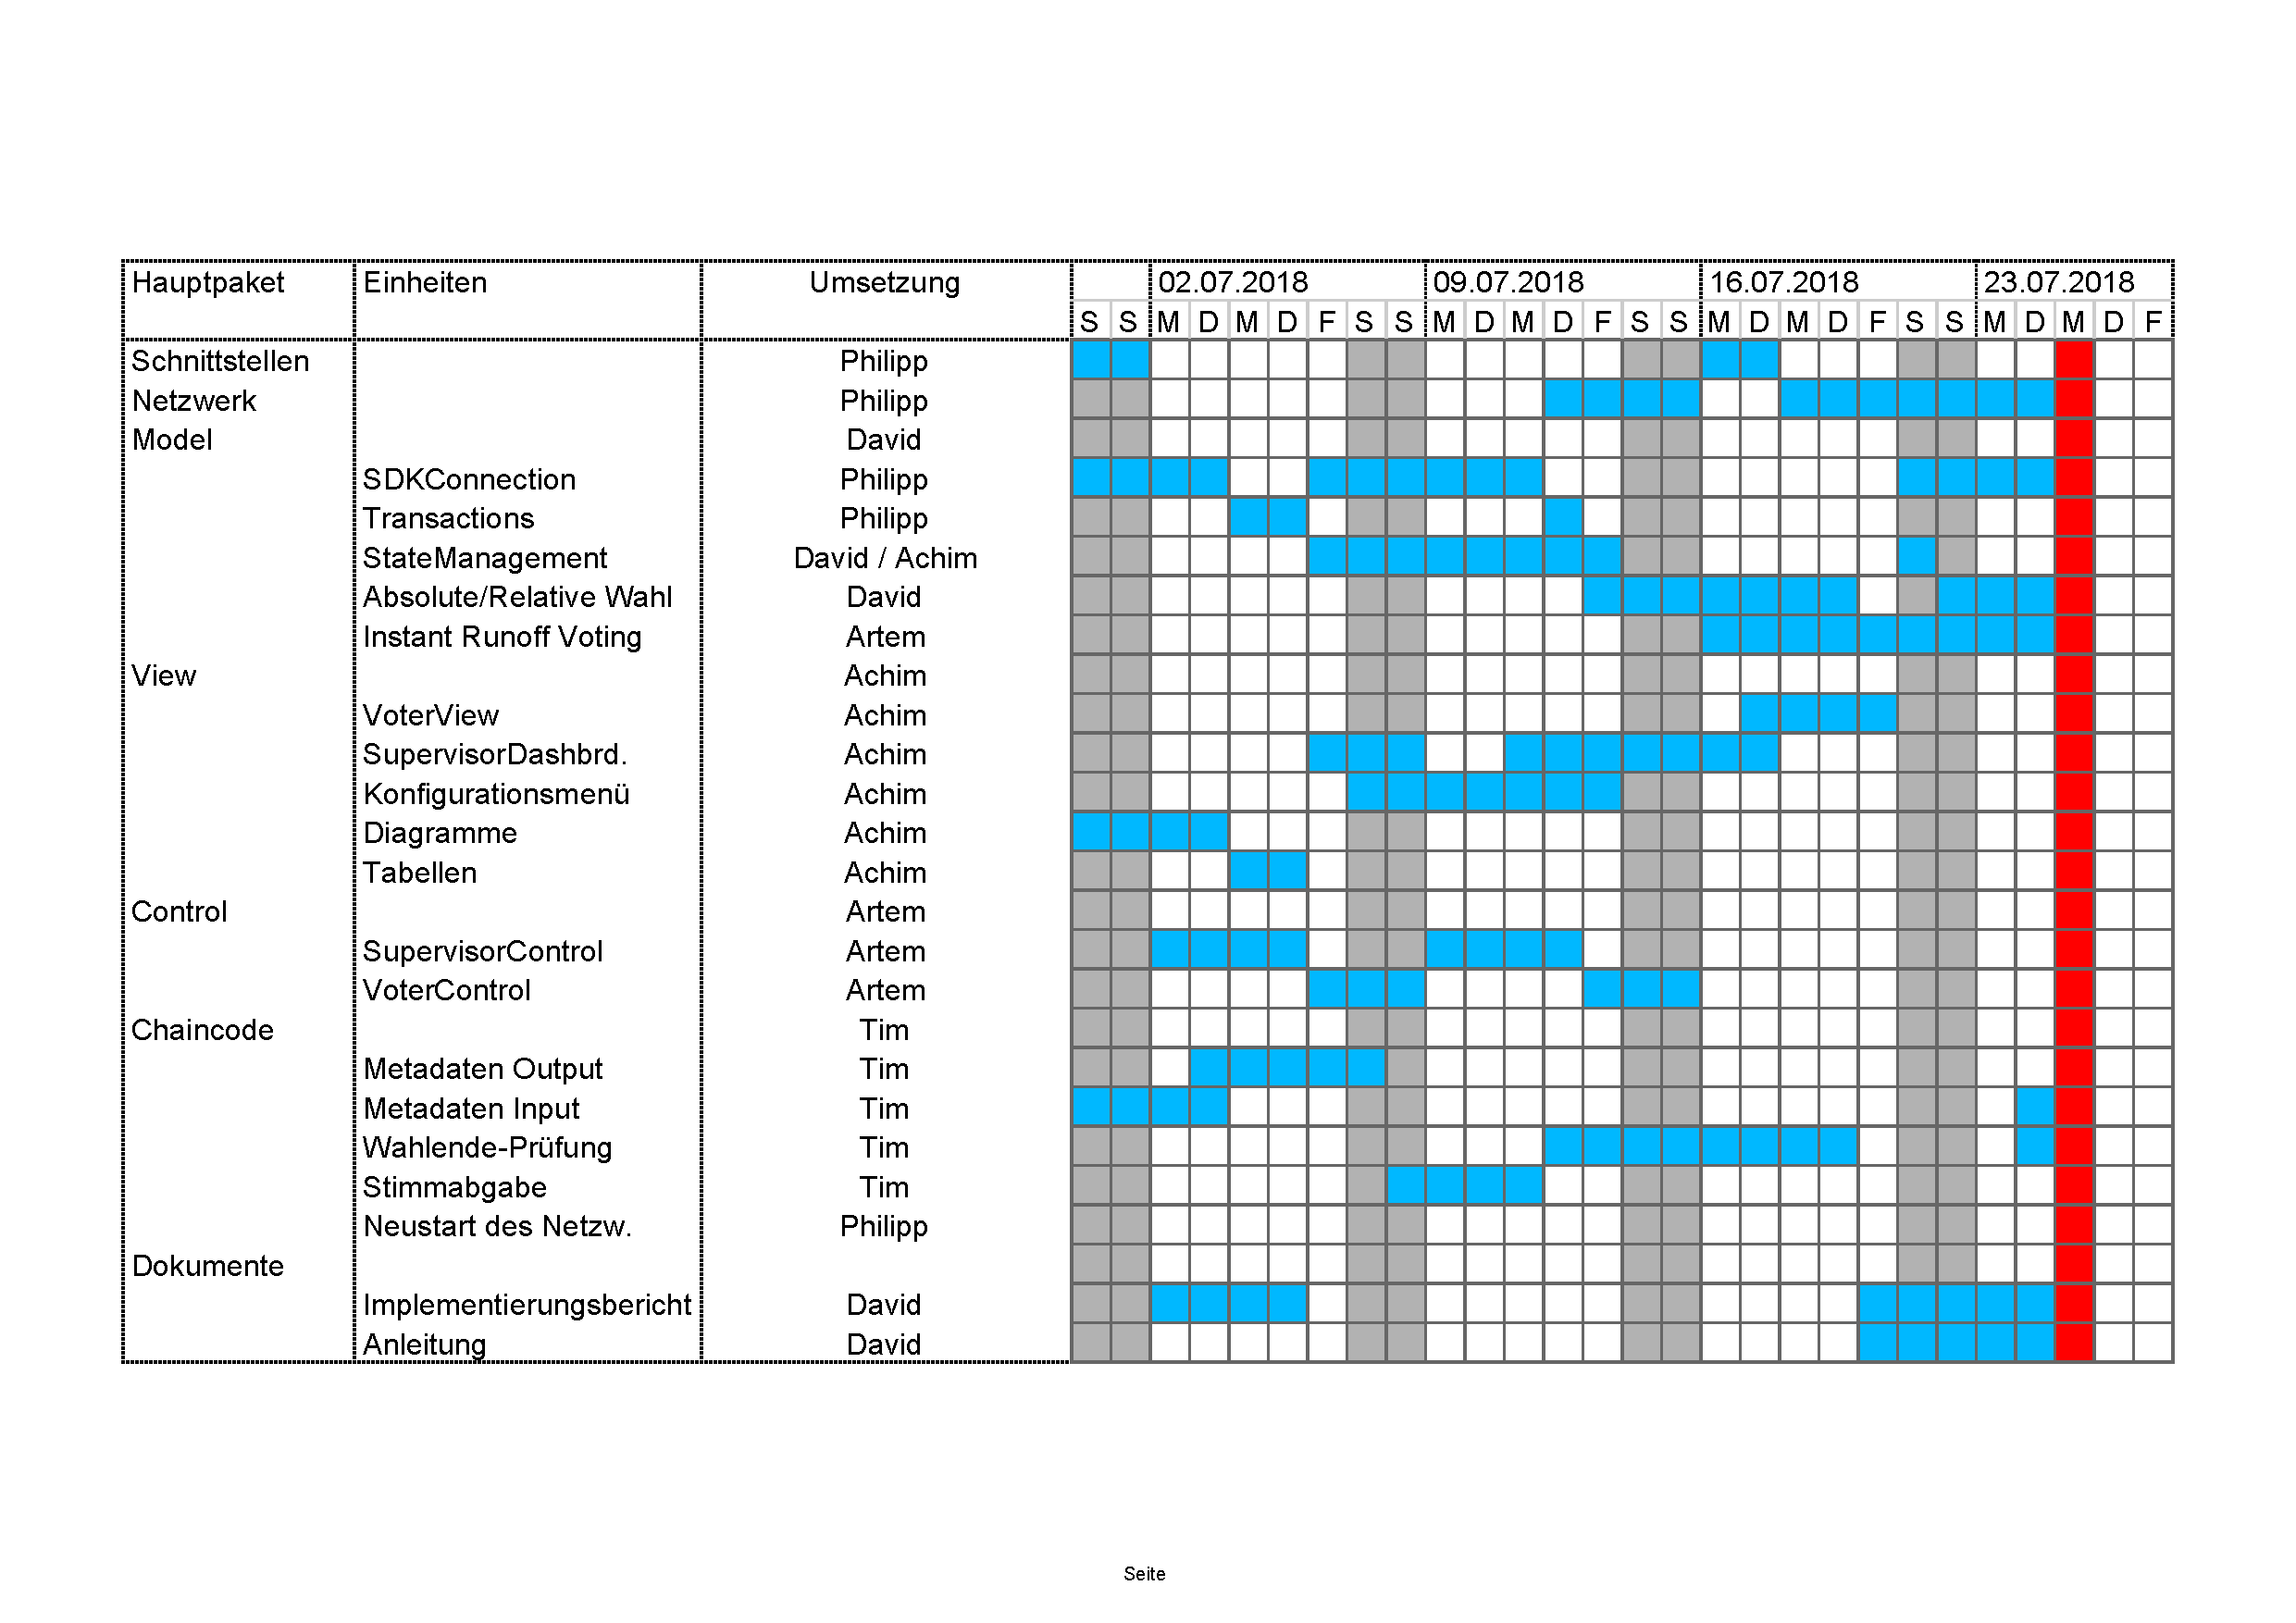
\includegraphics[width=\textwidth]{pictures/Gantt.pdf}
	\caption{Gantt-Diagramm (unvollständig)}
	\label{fig:gantt}
\end{figure}


\section{Umsetzung der funktionalen Anforderungen}

\subsection{Musskriterien}

\subsection{Sollkriterien}

\subsection{Kannkriterien}


\section{Umsetzung der nichtfunktionalen-Anforderungen}

\subsection{Produktleistungen}
	
\subsection{Weitere nichtfunktionale Anforderungen}

		
\section{Umsetzung von Entwurfsentscheidungen}


\section{Änderungen zum Entwurf}


\end{document}

